\section{preliminaries}\label{sec:pre}
In this section, we first introduce some preliminary information on general hash tables and  present background material on GPU architecture. Frequently used notations are summarized in Table~\ref{tbl:stat:datasets}.

\begin{table}
	\centering
	\caption{Frequently Used Notations}
	\vspace{-1em}
	\label{tbl:stat:datasets}
	\begin{tabular}{|c|l|}
		\hline
		$(k,v)$ & a key value pair \\ \hline
		$d$		& the number of hash functions \\ \hline
		$h^i$	& the $i$th hash table \\ \hline
		$|h^i|,n_i,m_i$	& range, table size and data size of $h^i$ \\ \hline
		$wid,l$	& a warp ID and the $l$th lane of the warp \\ \hline
		$\theta$& the filled factor of the entire hash table \\ \hline
		$\theta_i$& the filled factor of hash table $i$ \\ \hline
		$loc$	& a bucket in the hash table \\ \hline
	\end{tabular}
\end{table}

\subsection{Hash Table}
The hash table is a fundamental data structure that stores KV pairs $(k,v)$, and the value could refer to either actual data or a reference to the data.
Hash tables offer the following functionalities: \formal{insert}$(k,v)$, which stores $(k,v)$ in the hash table; \formal{find}$(k)$, in which the given $k$ values returns the associated values if they exist and NULL otherwise; and \formal{delete}$(k)$, which removes existing KV pairs that match $k$ if they are present in the table.

Given a hash function with range $0 \ldots h-1$, collisions must happen when we insert $m>h$ keys into the table. There are many schemes to resolve collisions: linear probing, quadratic probing, chaining and etc. Unlike these schemes, cuckoo hashing \cite{pagh2004cuckoo} guarantees a worst case constant complexity for \formal{find} and \formal{delete},  and an amortized constant complexity for \formal{insert}. A cuckoo hash uses multiple (i.e., $d$) hash tables with independent hash functions $h^1,h^2,\ldots,h^d$ and stores a KV pair in \emph{one} of the hash tables. When inserting $(k,v)$, we store the pair in $loc=h^1(k)$ and terminate if there is no element at this location. Otherwise, if there exists $k'$ such that $h^1(k')=loc$, $k'$ is evicted and then reinserted into another hash table, e.g., $loc'=h^2(k')$.
We repeat this process until encountering an empty location.

For a hash table with the hash function $h^i$, $|h^i|$ is defined to be the number of unique hash values for $h^i$ and $n_i$ to be the total memory size allocated for the hash table.
A location or a hash value for $h^i$ is represented as $loc = h^i_j$ where $j \in [0,|h^i|-1]$.
If the occupied space of the hash table is $m_i$, the filled factor of $h^i$ is denoted as $\theta_i = m_i / n_i$. The overall filled factor of the cuckoo hash table is thus denoted as $\theta = (\sum_i m_i) / (\sum_i n_i)$.

\subsection{GPU Architecture}

\begin{figure}[t]
	\centering
	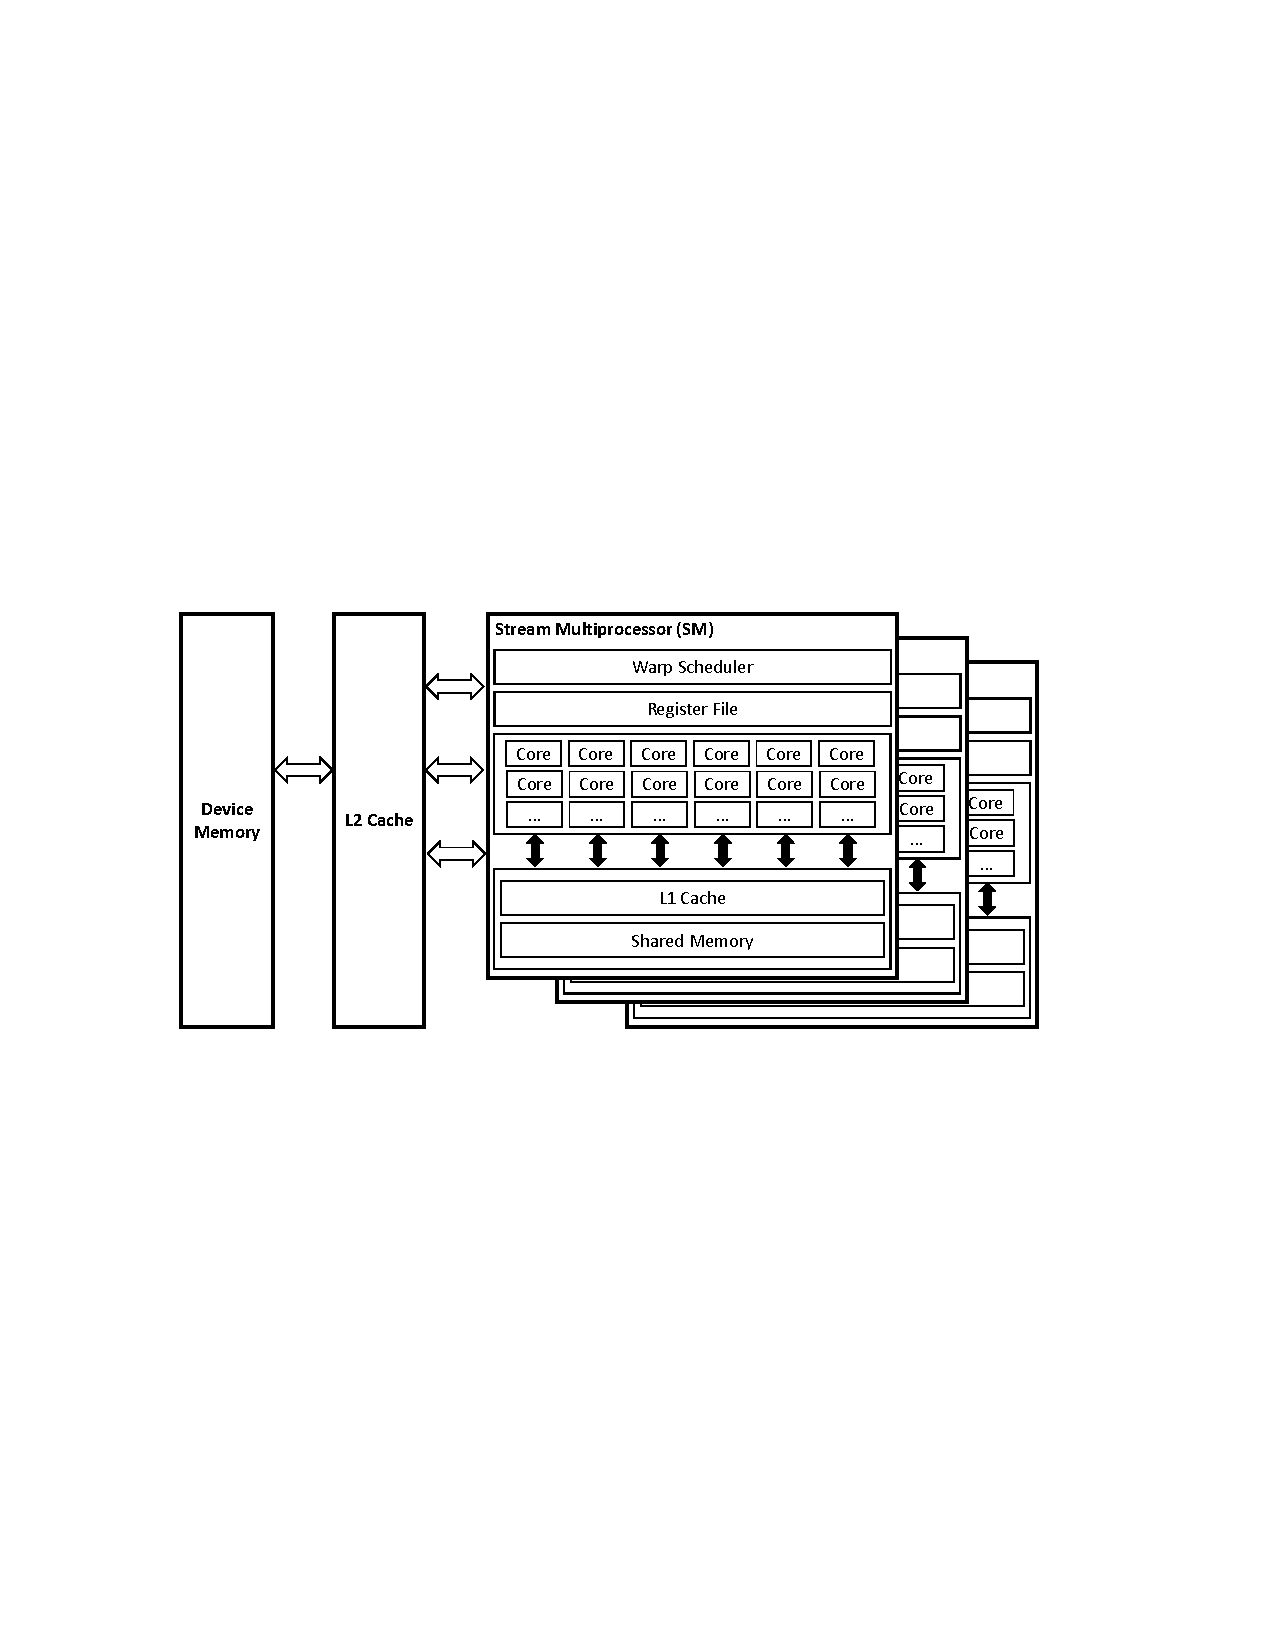
\includegraphics[width=0.5\textwidth]{fig/GPU-arch.pdf}
	\caption{Layout of an NVIDIA GPU architecture}
	\label{fig:arch}
\end{figure}

We introduce the background of the NVIDIA GPU architecture in this paper because its popularity and the wide adoption of the CUDA programming language. 
However, our proposed approaches are not unique to NVIDIA GPUs and can also be implemented on other GPU architectures. 
Figure~\ref{fig:arch} presents a high-level layout of a NVIDIA GPU. 
An application written in CUDA executes on GPUs by invoking the \emph{kernel} function. The kernel is organized as several \emph{thread blocks}, and one block executes all its threads on a \emph{streaming multiprocessor} (SM), which contains several CUDA cores as depicted in Figure~\ref{fig:arch}. Within each block, threads are divided into \emph{warps} of 32 threads each. 
A CUDA core executes the same instruction of a warp in lockstep.
Each warp runs independently, but warps can collaborate through different memory types as discussed in the following.  

\vspace{1mm}\noindent\textbf{Memory Hierarchy.} Compared with CPUs, GPUs are built with large register files that enable massive parallelism. 
%For example, NVIDIA GTX 1080 GPUs feature 256KB of register files for each SM. 
Furthermore, the shared memory, which has similar performance to L1 cache, can be programmed within a block to facilitate efficient memory access inside an SM.
The L2 cache is shared among all SMs to accelerate memory access to the device memory, which has the largest capacity and the lowest bandwidth in the memory hierarchy.

%GPUs offer an significant better data accessing throughputs than CPUs for two major reasons. 
%First,the device memory has high memory bandwidth, often an order of magnitude faster than RAM.
%Second, GPUs effectively hide memory access latency by warp switching. When a warp is blocked by memory accesses, other warps whose next instruction has its operands ready are eligible to be scheduled for execution. With sufficient threads launched, memory stalls can be minimized or even eliminated \cite{zhang2015mega}.
%Thus, the fast data accessing performance makes GPUs an ideal accelerator for data intensive applications such as hash tables. 

%Data is transferred between CPUs and GPUs (or between two GPU devices) via the PCIe link (Gen 3), which has been the bottleneck of many data-intensive applications \cite{zhang2015mega,kaldewey2012gpu,zhang2013omnidb}. In recent years, there have been many innovations proposed to reduce the overhead of the data transfer, from overlapping PCIe transfer with kernel execution to using hardware acceleration such as PCIe Gen 4 and NVlink \cite{thompto2016power9}. Nonetheless, we omit the discussion on how to minimize this data transfer cost since it is orthogonal to designing an efficient hash table on \emph{one} GPU device.

\vspace{1mm}\noindent\textbf{Optimizing GPU Programs.}
There are several important guidelines to harness the massive parallelism of GPUs.
\begin{itemize}
	\item \emph{Minimize Warp Divergence.} Threads in a warp will be serialized if executing different instructions. To enable maximum parallelism, one must minimize branching statements executed within a warp.  
	\item \emph{Coalesced Memory Access.} Warps have a wide cache line size. The threads are better off reading consecutive memory locations to fully utilize the device memory bandwidth, otherwise a single read instruction by a warp will trigger multiple random accesses. 
	\item \emph{Control Resource Usage.} Registers and shared memory are valuable resources for enabling fast memory accesses. Nevertheless, each SM has limited resources and overdosing register files or shared memory leads to reduced parallelism on an SM.  
	\item \emph{Atomic Operations.} When facing thread conflicts, an improper locking implementation causes serious performance degradation. One can leverage the native support of atomic operations \cite{sanders2010cuda} on GPUs to carefully resolve the conflicts and minimize thread spinning.
\end{itemize}